\documentclass{ctexart}

% --- 导入所需宏包 ---
\usepackage[a4paper, vmargin=2.5cm, hmargin=2cm]{geometry}
\usepackage{amsmath, amssymb, amsthm}
\usepackage[svgnames]{xcolor}
\usepackage[most]{tcolorbox}
\usepackage{fancyhdr}
\usepackage{lmodern} % 提供更多字体变体,包括粗斜体无衬线字体
\usepackage{tikz}
\usetikzlibrary{intersections, patterns, shadows, decorations.pathmorphing}
\usepackage{fontawesome5} % 更新的图标包
\usepackage{enumitem}
\usepackage{mdframed}
\usepackage{varwidth} % 需要用于 formulabox
\usepackage{background} % 用于添加水印
\usepackage{transparent} % 用于透明度控制
\usepackage{everypage} % 用于在每页添加前景水印

% --- 修复页眉高度警告 ---
\setlength{\headheight}{22pt}

% --- 水印设置 ---
\backgroundsetup{
    scale=1,
    color=black,
    opacity=0.15,
    angle=0,
    position=current page.center,
    vshift=0cm,
    hshift=0cm,
    contents={%
        \begin{tikzpicture}[remember picture, overlay]
            % 使用页面尺寸计算水印位置,确保完全覆盖
            % A4纸尺寸:210mm × 297mm,转换为cm约为21cm × 29.7cm
            \foreach \x in {-12,-8,-4,0,4,8,12} {
                \foreach \y in {-16,-12,-8,-4,0,4,8,12,16} {
                    % 30度倾斜,2.5倍正文字体大小的水印,提高层级
                    \node[rotate=30, text opacity=0.15, text=gray!70, font=\sffamily\bfseries] at (\x cm,\y cm) 
                        {\fontsize{30}{36}\selectfont 雪履千山客};
                }
            }
            % 添加额外的水印行,确保边缘也有覆盖
            \foreach \x in {-10,-6,-2,2,6,10} {
                \foreach \y in {-14,-10,-6,-2,2,6,10,14} {
                    \node[rotate=30, text opacity=0.12, text=gray!60, font=\sffamily] at (\x cm,\y cm) 
                        {\fontsize{24}{30}\selectfont 内部资料};
                }
            }
        \end{tikzpicture}
    }
}

% --- 前景水印设置(显示在所有内容之上)---
\AddEverypageHook{%
    \begin{tikzpicture}[remember picture, overlay]
        % 前景水印,显示在tcolorbox之上,透明度更高
        \foreach \x in {-12,-8,-4,0,4,8,12} {
            \foreach \y in {-16,-12,-8,-4,0,4,8,12,16} {
                \node[rotate=30, text opacity=0.15, text=gray!50, font=\sffamily\bfseries] at (\x cm,\y cm) 
                    {\fontsize{32}{38}\selectfont 雪履千山客};
            }
        }
        % 添加更多水印层确保覆盖
        \foreach \x in {-10,-6,-2,2,6,10} {
            \foreach \y in {-14,-10,-6,-2,2,6,10,14} {
                \node[rotate=30, text opacity=0.12, text=gray!45, font=\sffamily] at (\x cm,\y cm) 
                    {\fontsize{26}{32}\selectfont 内部资料};
            }
        }
    \end{tikzpicture}
}

% --- 自定义优雅颜色定义 ---
\definecolor{themeblue}{RGB}{52, 73, 94}%主题蓝
\definecolor{elegantpurple}{RGB}{155, 89, 182}%优雅紫
\definecolor{warmorange}{RGB}{230, 126, 34}%温暖橙
\definecolor{forestgreen}{RGB}{39, 174, 96}%森林绿
\definecolor{deepblue}{RGB}{41, 128, 185}%深邃蓝
\definecolor{sunsityellow}{RGB}{241, 196, 15}%阳光黄
\definecolor{lightgrayblue}{RGB}{236, 240, 241}%浅灰蓝
\definecolor{softpink}{RGB}{250, 219, 216}%柔和粉
\definecolor{crimsonred}{RGB}{220, 20, 60}%深红
\definecolor{darkslategray}{RGB}{47, 79, 79}%深石板灰
\definecolor{lightgreen}{RGB}{144, 238, 144}%浅绿色
\definecolor{gree}{RGB}{101, 191, 127}%绿色浅
\definecolor{gre}{RGB}{101, 191, 127}%绿色浅(别名)
\definecolor{notegreen}{RGB}{7, 135, 44}%注意绿
\definecolor{green}{RGB}{34, 139, 34}%标准绿色

% --- 页面布局与页眉页脚设置 ---
\pagestyle{fancy}
\fancyhf{}
\fancyhead[L]{\color{crimsonred}\textbf{\faBook\ 高中数学讲义}}
\fancyhead[R]{\color{crimsonred}\textit{Professional Mathematics \faUser}}
\fancyfoot[C]{\color{crimsonred!70}\small\textbf{--\ \thepage\ --}}
\renewcommand{\headrulewidth}{1pt}
\renewcommand{\footrulewidth}{0pt}
\renewcommand{\headrule}{\hbox to\headwidth{\color{crimsonred!30}\leaders\hrule height \headrulewidth\hfill}}

% --- 自定义优美的文本框环境 ---

% 主标题框 (斜体英文+中文,专业设计)
\newtcolorbox{chaptertitle}[2]{
    enhanced,
    colback=themeblue!8!white,
    colframe=white,
    boxrule=0pt,
    arc=0pt,
    outer arc=0pt,
    width=0.90\textwidth,
    fonttitle=\Huge\sffamily,
    title={\makebox[1.8em][l]{\textcolor{themeblue}{#1}}\ \textbf{\textit{{#2}}}},
    coltitle=themeblue,
    center title,
    toptitle=0pt,
    bottomtitle=0pt,
    before skip=0pt,
    after skip=0pt
}

% 习题框 (新样式设计,六边形标题框)
\newtcolorbox{exercisebox}[1]{
    enhanced,
    title={\makebox[1.8em][l]{\textcolor{forestgreen}{\faEdit}}\ \textit{Exercise} #1},
    colframe=forestgreen!50!black,
    colback=forestgreen!10!white,
    colbacktitle=forestgreen!5!yellow!10!white,
    fonttitle=\bfseries,
    coltitle=black,
    attach boxed title to top center={yshift=-0.25mm-\tcboxedtitleheight/2,yshifttext=2mm-\tcboxedtitleheight/2},
    boxed title style={boxrule=0.5mm,
        frame code={ \path[tcb fill frame] ([xshift=-4mm]frame.west)
            -- (frame.north west) -- (frame.north east) -- ([xshift=4mm]frame.east)
            -- (frame.south east) -- (frame.south west) -- cycle; },
        interior code={ \path[tcb fill interior] ([xshift=-2mm]interior.west)
            -- (interior.north west) -- (interior.north east)
            -- ([xshift=2mm]interior.east) -- (interior.south east) -- (interior.south west)
            -- cycle;} },
    left=15pt, right=10pt, top=15pt, bottom=10pt,
    before skip=20pt, after skip=15pt,
    breakable
}

% 解析框 (专业方正设计,左侧竖线,优化对齐)
\newtcolorbox{analysisbox}{
    enhanced,
    colback=elegantpurple!5!white,
    colframe=white,
    boxrule=0pt,
    arc=0pt,
    outer arc=0pt,
    fonttitle=\sffamily,
    title={\makebox[1.8em][l]{\textcolor{elegantpurple}{\faLightbulb}}\ \textit{Analysis}},
    coltitle=elegantpurple!90!white,
    colbacktitle=elegantpurple!35!white,
    attach boxed title to top left={yshift=-2mm, xshift=3mm},
    boxed title style={arc=0pt, outer arc=0pt, frame hidden},
    borderline west={1pt}{0pt}{elegantpurple},
    left=15pt, right=10pt, top=15pt, bottom=10pt,
    before skip=20pt, after skip=15pt,
    breakable
}

% 拓展框 (新样式设计,带斜角标题框)
\newtcolorbox{expandbox}[1][]{
    enhanced,
    skin=enhancedlast jigsaw,
    attach boxed title to top left={xshift=-4mm,yshift=-0.5mm},
    fonttitle=\bfseries\sffamily,
    varwidth boxed title=0.7\linewidth,
    colbacktitle=blue!45!white,
    colframe=red!50!black,
    interior style={top color=blue!10!white,bottom color=red!10!white},
    boxed title style={empty,arc=0pt,outer arc=0pt,boxrule=0pt},
    underlay boxed title={
        \fill[blue!45!white] (title.north west) -- (title.north east)
        -- +(\tcboxedtitleheight-1mm,-\tcboxedtitleheight+1mm)
        -- ([xshift=4mm,yshift=0.5mm]frame.north east) -- +(0mm,-1mm)
        -- (title.south west) -- cycle;
        \fill[blue!45!white!50!black] ([yshift=-0.5mm]frame.north west)
        -- +(-0.4,0) -- +(0,-0.3) -- cycle;
        \fill[blue!45!white!50!black] ([yshift=-0.5mm]frame.north east)
        -- +(0,-0.3) -- +(0.4,0) -- cycle; 
    },
    title={\makebox[1.8em][l]{\textcolor{warmorange}{\faRocket}}\ \textit{Extension}},
    left=15pt, right=10pt, top=15pt, bottom=10pt,
    before skip=20pt, after skip=15pt,
    breakable,
    #1
}

% 定理框 (新增,优雅设计)
\newtcolorbox{theorembox}[1]{
    enhanced,
    colback=deepblue!8!white,
    colframe=white,
    boxrule=0pt,
    arc=0pt,
    outer arc=0pt,
    fonttitle=\sffamily,
    title={\makebox[1.8em][l]{\textcolor{deepblue}{\faGraduationCap}}\ \textit{Theorem} },
    coltitle=deepblue!90!white,
    colbacktitle=deepblue!35!white,
    attach boxed title to top left={yshift=-2mm, xshift=3mm},
    boxed title style={arc=0pt, outer arc=0pt, frame hidden},
    borderline west={1pt}{0pt}{deepblue},
    left=15pt, right=10pt, top=15pt, bottom=10pt,
    before skip=20pt, after skip=15pt,
    breakable,
    overlay={%
        \node[rotate=30, text opacity=0.08, text=gray!30, font=\sffamily] at (2,1) 
            {\fontsize{16}{20}\selectfont 雪履千山客};
        \node[rotate=30, text opacity=0.06, text=gray!25, font=\sffamily] at (-1,0) 
            {\fontsize{14}{18}\selectfont 内部资料};
    }
}

% 注意事项框 (新样式设计,渐变标题)
\newtcolorbox{notebox}{
    colback=white,
    title={\makebox[1.8em][l]{\textcolor{crimsonred}{\faExclamationTriangle}}\ \textit{Note}},
    colframe=white,
    boxrule=0pt,
    enhanced,
    title style={left color=crimsonred!50,right color=white,middle color=white},
    arc=0mm,
    titlerule=0pt,
    fonttitle=\bfseries\sffamily,
    left=15pt, right=10pt, top=15pt, bottom=10pt,
    before skip=20pt, after skip=15pt,
    breakable
}

% 公式盒子 (新增,红色主题)
\newtcolorbox{formulabox}[1]{
    enhanced,
    colback=red!10!white,
    colframe=red!50!black,
    boxrule=1.5pt,
    arc=3pt,
    fonttitle=\bfseries\sffamily\color{red!50!black},
    colbacktitle=blue!45!white,
    attach boxed title to top left={yshift=-2mm, xshift=3mm},
    boxed title style={arc=0pt, outer arc=0pt, frame hidden},
    borderline west={2pt}{0pt}{red!50!black},
    left=15pt, right=10pt, top=15pt, bottom=10pt,
    before skip=20pt, after skip=15pt,
    breakable,
    title={#1},
    overlay={%
        \node[rotate=30, text opacity=0.06, text=gray!25, font=\sffamily] at (3,2) 
            {\fontsize{14}{18}\selectfont 雪履千山客};
        \node[rotate=30, text opacity=0.05, text=gray!20, font=\sffamily] at (-2,-1) 
            {\fontsize{12}{16}\selectfont 内部资料};
    }
}

% 例题盒子 (新增,绿色主题)
\newtcolorbox{exampleBox}[1]{
    enhanced,
    colback=lightgreen!10!white,
    colframe=green!70!black,
    boxrule=1.5pt,
    arc=3pt,
    fonttitle=\bfseries\sffamily\color{green!70!black},
    colbacktitle=green!20!white,
    attach boxed title to top left={yshift=-2mm, xshift=3mm},
    boxed title style={arc=0pt, outer arc=0pt, frame hidden},
    borderline west={2pt}{0pt}{green!70!black},
    left=15pt, right=10pt, top=15pt, bottom=10pt,
    before skip=20pt, after skip=15pt,
    breakable,
    title={#1},
    overlay={%
        \node[rotate=30, text opacity=0.06, text=gray!25, font=\sffamily] at (4,3) 
            {\fontsize{14}{18}\selectfont 雪履千山客};
        \node[rotate=30, text opacity=0.05, text=gray!20, font=\sffamily] at (-2,1) 
            {\fontsize{12}{16}\selectfont 内部资料};
        \node[rotate=30, text opacity=0.04, text=gray!15, font=\sffamily] at (1,-2) 
            {\fontsize{10}{14}\selectfont 专属};
    }
}

% --- 数学公式和排版优化 ---
\renewcommand{\arraystretch}{1.4}
\setlength{\jot}{8pt}

% 自定义数学命令
\newcommand{\highlight}[1]{\colorbox{sunsityellow!20}{\ensuremath{#1}}}
\newcommand{\result}[1]{\tcbhighmath[colback=deepblue!15, colframe=deepblue, arc=3pt]{#1}}
\newcommand{\important}[1]{\textcolor{crimsonred}{\textbf{#1}}}

% --- 文档开始 ---
\begin{document}
\thispagestyle{fancy}

% 优美的章节标题 (主标题斜体英文+中文)
\begin{center}
    \begin{chaptertitle}{\faBookOpen}{Analytic Geometry 4.1}
    \end{chaptertitle}
\end{center}


\begin{theorembox}{4.1}
\textbf{圆锥曲线的统一定义:} 平面内与一定点(焦点)和一条定直线(准线)的距离比为常数 $e$(离心率)的点的轨迹称为圆锥曲线。

当 $0 < e < 1$ 时为椭圆;当 $e = 1$ 时为抛物线;当 $e > 1$ 时为双曲线。
\end{theorembox}

% 公式盒子样例
\begin{formulabox}{椭圆的重要公式}
\textbf{标准椭圆 $\frac{x^2}{a^2} + \frac{y^2}{b^2} = 1$ 的重要公式:}

\begin{enumerate}[leftmargin=15pt, itemsep=6pt]
    \item \textbf{离心率:} $e = \frac{c}{a} = \sqrt{1 - \frac{b^2}{a^2}}$,其中 $c^2 = a^2 - b^2$
    
    \item \textbf{焦点坐标:} $F_1(-c, 0)$,$F_2(c, 0)$
    
    \item \textbf{准线方程:} $x = \pm\frac{a^2}{c}$
    
    \item \textbf{焦点弦长公式:} 过焦点的弦长 $|AB| = \frac{2b^2}{a} \cdot \frac{1}{1 - e^2\cos^2\theta}$
    
    \item \textbf{切线方程:} 椭圆上点 $(x_0, y_0)$ 处的切线方程为 $\frac{x_0 x}{a^2} + \frac{y_0 y}{b^2} = 1$
\end{enumerate}

\highlight{\text{特别提醒:椭圆的离心率越小,椭圆越接近圆形}}
\end{formulabox}

% 例题盒子样例
\begin{exampleBox}{例题:椭圆的焦点弦性质}
\textbf{题目:} 已知椭圆 $C: \frac{x^2}{9} + \frac{y^2}{5} = 1$,$F$ 为其右焦点,直线 $l$ 过点 $F$ 且倾斜角为 $60^\circ$,求直线 $l$ 与椭圆 $C$ 的交点弦长。

\medskip
\textbf{解题分析:}

\textit{Step 1:} 确定椭圆参数
\begin{itemize}[leftmargin=15pt, itemsep=4pt]
    \item $a^2 = 9$,$b^2 = 5$,故 $a = 3$,$b = \sqrt{5}$
    \item $c^2 = a^2 - b^2 = 9 - 5 = 4$,故 $c = 2$
    \item 右焦点 $F(2, 0)$,离心率 $e = \frac{2}{3}$
\end{itemize}

\textit{Step 2:} 求直线方程
\begin{itemize}[leftmargin=15pt, itemsep=4pt]
    \item 直线 $l$ 的斜率为 $k = \tan 60^\circ = \sqrt{3}$
    \item 直线方程:$y = \sqrt{3}(x - 2)$
\end{itemize}

\textit{Step 3:} 联立求解
联立 $\begin{cases} y = \sqrt{3}(x - 2) \\ \frac{x^2}{9} + \frac{y^2}{5} = 1 \end{cases}$

化简得:$8x^2 - 18x + 9 = 0$

\textit{Step 4:} 计算弦长
由韦达定理:$x_1 + x_2 = \frac{9}{4}$,$x_1 x_2 = \frac{9}{8}$

弦长 $|AB| = \sqrt{1 + k^2} \cdot |x_1 - x_2| = 2\sqrt{(x_1 + x_2)^2 - 4x_1 x_2} = 2\sqrt{\frac{81}{16} - \frac{9}{2}} = \frac{3}{2}$

\result{\textbf{答案:}弦长为 \frac{3}{2}}
\end{exampleBox}

\begin{exercisebox}{4.1}
已知椭圆 $\frac{x^2}{a^2} + \frac{y^2}{b^2} = 1$ (其中 $a > b > 0$) 的离心率为 $\frac{\sqrt{3}}{2}$,且过点 $(2, 1)$。

(1) 求椭圆的标准方程;

(2) 设直线 $l: y = kx + m$ 与椭圆相交于 $A$、$B$ 两点,若 $A$、$B$ 关于直线 $y = 2x$ 对称,求直线 $l$ 的方程。
\end{exercisebox}

\begin{analysisbox}
\textbf{\color{elegantpurple}\textit{Solution Strategy} \quad 解题思路:}

\begin{enumerate}[leftmargin=15pt, itemsep=8pt]
    \item \textbf{第一问:} 利用离心率公式 $e = \frac{c}{a}$ 和椭圆过定点条件建立方程组
    
    \item \textbf{第二问:} 利用对称性质,若两点关于直线对称,则:
    
    \begin{itemize}
        \item 连线中点在对称轴上
        \item 连线斜率与对称轴斜率乘积为 $-1$
    \end{itemize}
\end{enumerate}

\medskip
\textbf{\color{elegantpurple}\textit{Detailed Calculation} \quad 具体计算:}

\textbf{第一问:} 由 $e = \frac{\sqrt{3}}{2}$,得 $\frac{c}{a} = \frac{\sqrt{3}}{2}$,即 $c^2 = \frac{3a^2}{4}$。

由 $c^2 = a^2 - b^2$,得 $b^2 = a^2 - c^2 = \frac{a^2}{4}$。

椭圆过点 $(2, 1)$,代入得:$\frac{4}{a^2} + \frac{1}{b^2} = 1$

将 $b^2 = \frac{a^2}{4}$ 代入:$\frac{4}{a^2} + \frac{4}{a^2} = 1$

解得 $a^2 = 8$,$b^2 = 2$。

\result{\text{椭圆方程:} \frac{x^2}{8} + \frac{y^2}{2} = 1}

\textbf{第二问:} 设 $A(x_1, y_1)$,$B(x_2, y_2)$,中点 $M\left(\frac{x_1+x_2}{2}, \frac{y_1+y_2}{2}\right)$。

由对称性质:
\begin{align}
&\text{中点在对称轴上:} \frac{y_1+y_2}{2} = 2 \cdot \frac{x_1+x_2}{2} \\
&\text{斜率关系:} k \cdot 2 = -1,\text{即} k = -\frac{1}{2}
\end{align}

联立椭圆方程与直线方程,利用韦达定理可得:
\result{y = -\frac{1}{2}x + 1}
\end{analysisbox}

\begin{notebox}
\important{解题要点:}
\begin{itemize}[leftmargin=15pt, itemsep=5pt]
    \item 对称问题的核心在于利用对称轴的性质
    \item 椭圆离心率 $e = \frac{c}{a}$ 是连接 $a$、$b$、$c$ 的桥梁
    \item 联立方程时要注意判别式 $\Delta > 0$ 的条件
\end{itemize}
\end{notebox}

\begin{figure}[h!]
\centering
\begin{tikzpicture}[scale=0.8, >=stealth]
    % 定义椭圆参数
    \def\a{2.83} % sqrt(8)
    \def\b{1.41} % sqrt(2)
    
    % 绘制坐标轴
    \draw[->] (-4,0) -- (4,0) node[right] {$x$};
    \draw[->] (0,-2.5) -- (0,2.5) node[above] {$y$};
    
    % 绘制椭圆
    \draw[thick, blue] (0,0) ellipse ({\a} and {\b});
    
    % 绘制对称轴
    \draw[dashed, red, thick] (-3,-6) -- (2,4) node[above] {$y = 2x$};
    
    % 绘制直线l
    \draw[green, thick] (-2,2) -- (4,-1) node[right] {$l: y = -\frac{1}{2}x + 1$};
    
    % 标记交点
    \coordinate (A) at (-1.6, 1.8);
    \coordinate (B) at (2.4, -0.2);
    \fill[green] (A) circle (2pt) node[above left] {$A$};
    \fill[green] (B) circle (2pt) node[below right] {$B$};
    
    % 标记中点
    \coordinate (M) at (0.4, 0.8);
    \fill[red] (M) circle (2pt) node[above] {$M$};
    
    % 标记原点和关键点
    \fill (0,0) circle (1.5pt) node[below left] {$O$};
    \fill (2,1) circle (2pt) node[above right] {$(2,1)$};
    
    % 添加网格
    \draw[gray!30, very thin] (-4,-2) grid (4,2);
    
\end{tikzpicture}
\caption{\textcolor{themeblue}{\textbf{\textit{Figure 4.1 - Ellipse and Symmetric Line} \quad 图 4.1 - 椭圆与对称直线}}}
\label{fig:ellipse}
\end{figure}

\begin{expandbox}
\textbf{拓展思考:}

\begin{enumerate}[leftmargin=15pt, itemsep=8pt]
    \item \textbf{一般化问题:} 若椭圆上两点关于直线 $y = kx + c$ 对称,如何求解?
    
    \item \textbf{双曲线情形:} 类似问题在双曲线中如何处理?
    
    \item \textbf{参数方程法:} 利用椭圆的参数方程 $\begin{cases} x = a\cos\theta \\ y = b\sin\theta \end{cases}$ 求解对称问题
\end{enumerate}

\textbf{相关定理:}
\begin{itemize}[leftmargin=15pt, itemsep=5pt]
    \item 焦点弦性质:过焦点的弦具有特殊的调和性质
    \item 切线方程:椭圆上一点的切线方程为 $\frac{x_0 x}{a^2} + \frac{y_0 y}{b^2} = 1$
\end{itemize}
\end{expandbox}

\newpage

% 第二个主题
\begin{center}
    \begin{chaptertitle}{\faInfinity}{Infinite Series 5.2}
    \end{chaptertitle}
\end{center}

% 数列公式盒子样例
\begin{formulabox}{数列与级数的重要公式}
\textbf{递推数列与无穷级数的核心公式:}

\begin{enumerate}[leftmargin=15pt, itemsep=6pt]
    \item \textbf{等差数列:} $a_n = a_1 + (n-1)d$,$S_n = \frac{n(a_1 + a_n)}{2} = \frac{n[2a_1 + (n-1)d]}{2}$
    
    \item \textbf{等比数列:} $a_n = a_1 \cdot q^{n-1}$,$S_n = \begin{cases} 
        na_1 & \text{若 } q = 1 \\
        \frac{a_1(1-q^n)}{1-q} & \text{若 } q \neq 1
    \end{cases}$
    
    \item \textbf{无穷等比级数:} $\sum_{n=1}^{\infty} a_1 q^{n-1} = \frac{a_1}{1-q}$ (当 $|q| < 1$ 时收敛)
    
    \item \textbf{调和级数:} $\sum_{n=1}^{\infty} \frac{1}{n}$ 发散,但 $\sum_{n=1}^{\infty} \frac{1}{n^2} = \frac{\pi^2}{6}$
    
    \item \textbf{递推关系变换:} 对于 $a_{n+1} = f(a_n)$ 型递推,常用换元法:
    \begin{itemize}
        \item 取倒数:$b_n = \frac{1}{a_n}$
        \item 线性变换:$b_n = a_n + c$ 或 $b_n = ka_n$
    \end{itemize}
\end{enumerate}

\highlight{\text{技巧提示:遇到分式递推时,优先考虑取倒数变换}}
\end{formulabox}

\begin{exercisebox}{5.1}
设数列 $\{a_n\}$ 满足 $a_1 = 1$,$a_{n+1} = \frac{2a_n}{a_n + 2}$ $(n \geq 1)$。

(1) 证明:$\frac{1}{a_n}$ 是等差数列;

(2) 求数列 $\{a_n\}$ 的通项公式;

(3) 求 $\sum_{n=1}^{\infty} a_n$ 的值。
\end{exercisebox}

% 例题盒子样例 - 数列求和
\begin{exampleBox}{例题:无穷级数的收敛性判断}
\textbf{题目:} 判断级数 $\sum_{n=1}^{\infty} \frac{(-1)^{n+1}}{n^2 + 1}$ 的收敛性,并求其近似值(精确到小数点后3位)。

\medskip
\textbf{解题过程:}

\textit{Step 1:} 判断收敛性
这是一个交错级数,形式为 $\sum_{n=1}^{\infty} (-1)^{n+1} u_n$,其中 $u_n = \frac{1}{n^2 + 1}$。

检验 Leibniz 判别法条件:
\begin{itemize}[leftmargin=15pt, itemsep=4pt]
    \item $u_n > 0$ 对所有 $n \geq 1$ 成立
    \item $u_{n+1} < u_n$:$\frac{1}{(n+1)^2 + 1} < \frac{1}{n^2 + 1}$ 成立
    \item $\lim_{n \to \infty} u_n = \lim_{n \to \infty} \frac{1}{n^2 + 1} = 0$
\end{itemize}

\textit{Step 2:} 绝对收敛性判断
$\sum_{n=1}^{\infty} |u_n| = \sum_{n=1}^{\infty} \frac{1}{n^2 + 1}$

由于 $\frac{1}{n^2 + 1} < \frac{1}{n^2}$ 且 $\sum_{n=1}^{\infty} \frac{1}{n^2}$ 收敛,故原级数绝对收敛。

\textit{Step 3:} 近似计算
计算前10项和:$S_{10} = \sum_{n=1}^{10} \frac{(-1)^{n+1}}{n^2 + 1} \approx 0.915$

\result{\textbf{结论:}级数绝对收敛,近似值为 0.915}
\end{exampleBox}

\begin{analysisbox}
\textbf{\color{elegantpurple}\textit{Analysis Method} \quad 分析方法:}

这是典型的递推数列问题,关键在于找到合适的变换使得新数列具有简单的递推关系。

\textbf{第一问:} 对递推关系取倒数:
$$\frac{1}{a_{n+1}} = \frac{a_n + 2}{2a_n} = \frac{1}{2} + \frac{1}{a_n}$$

设 $b_n = \frac{1}{a_n}$,则 $b_{n+1} = b_n + \frac{1}{2}$,$b_1 = 1$。

显然 $\{b_n\}$ 是首项为 $1$,公差为 $\frac{1}{2}$ 的等差数列。

\textbf{第二问:} 
$$b_n = 1 + (n-1) \cdot \frac{1}{2} = \frac{n+1}{2}$$

因此:\result{a_n = \frac{1}{b_n} = \frac{2}{n+1}}

\textbf{第三问:} 
$$\sum_{n=1}^{\infty} a_n = \sum_{n=1}^{\infty} \frac{2}{n+1} = 2\sum_{n=2}^{\infty} \frac{1}{n}$$

由于调和级数 $\sum_{n=1}^{\infty} \frac{1}{n}$ 发散,所以原级数发散。

\result{\textbf{答案:}级数发散}
\end{analysisbox}

\begin{notebox}
\important{解题关键点:}
\begin{itemize}[leftmargin=15pt, itemsep=5pt]
    \item 递推数列问题优先考虑变量替换
    \item 取倒数是处理分式递推的常用技巧
    \item 判断级数收敛性要结合具体的判别法
\end{itemize}
\end{notebox}

\end{document}